%!TEX root = ../main.tex
\subsection{Analysis}
\label{sub:controller_board_analysis}

In order to develop a controller board capable of controlling a double pendulum, the required functionality of the board needs to be determined. 
This section will constitute an analysis of this functionality and of possible solutions to desired functionality.

\subsubsection{Communication} % (fold)
\label{ssub:communication}
The controller board should be able to communicate wirelessly with the joints as discussed in section \ref{ssub:mechanics}.
The wireless link should provide sufficient bandwidth that the angular position of the joint can be transmitted sufficiently frequently.
From section \ref{ssub:encoder} it can be seen that the encoder chosen for the joints allows 7200 counts per revolution.
This can be represented using 13 bit. 
Adding a 3 bit identifier makes the payload of a message 16 bit.
This is a rough estimate which will be used for the purposes of this analysis.
A number of different protocols exist which could be used in this project.
Three were under consideration for this project:
\begin{itemize}
	\item \textbf{TCP/IP over WiFi:} TCP/IP is the defacto standard for communication between computers, both wired and wirelessly.
	This, along with the very large throughput, makes it an enticing option.
	Considering the rather small message size this protocol does impose a significant amount of overhead.
	In addition to the communication overhead, TCP/IP also requires some form of driver, making it difficult to forego the use of Linux in the joints, an OS that increases the requirements to the processing unit in the joint considerably.
	\item \textbf{Bluetooth:} The Bluetooth protocol is developed specifically for low power, short range data transmission and is used extensively in various mobile applications \cite{bluetooth}.
	As with the previous option, a considerable amount of overhead is required in setting up bluetooth as well as in the transmission of packets, making it less desirable.
	\item \textbf{Radio Frequency:} While not strictly a protocol, using an RF transceiver eliminates the additional overhead associated with the previously mentioned protocols.
	RF transceivers come with a number of different interfaces such as SPI or I2C and will simply transmit the data received through that interface.
	This makes it easy to communicate using this method through bare-metal code or even VHDL.
\end{itemize}
Considering the above it was chosen to use an RF transceiver to facilitate the communication between the joints and the controller board.
An RF transceiver can be implemented using very low power, making it ideal for the battery powered joints.
% subsubsection communication (end)

\subsubsection{The MicroZed Development Platform} % (fold)
\label{ssub:microcontroller}
The MicroZed \cite{microzed} development platform is a Zynq-7000 series based platform which the authors have worked extensively with in previous projects \cite{isaswarm}.
It was developed by Avnet specifically to be implemented in a product and as such there are fewer built-in features to the board, resulting in a reasonably small footprint and an efficient interface.
Most of the design done by the authors in \cite{isaswarm} can be reused with limited modifications.
For these reasons the MicroZed will be used in this project.
\\~\\
One thing of note is that the Zynq-7000 series of chips requires a specific startup/shutdown sequency, detailed in \cite{carrier_card_design_guide}, which ensures that signal integrity is maintained during startup and shutdown of the platform.
This functionality should also be verified in this project.
% subsubsection microcontroller (end)

\subsubsection{Motor Driver}
It is necessary to device some form of driving circuitry for the motor driving the timing belt.
The motor should be able to move in both directions. 
An H-bridge allows this bidirectional movement.
By properly switching the MOSFETs in the bridge the average voltage across the motor can be controlled and therefore also the speed and direction of the motor.
As such, an H-bridge must be designed for the controller board. 
This will in turn require that an H-bridge driver circuit is designed.

\subsubsection{Capacitor Bank} % (fold)
From simulation it was found that a capacitor bank across the supply near the H-bridge is required in order to protect the remainder of the PCB against ripple current and voltage spikes.
See section \ref{ssub:sup_caps} for an in depth discussion.
The necessary amount of supply capacitance must be determined.
\\~\\
When introducing a large amount of capacitance in a circuit, a problem known as inrush current arises \cite{inrush}.
This happens when the circuit is powered on and the initial charging of the capacitors occur.
Due to the amount of capacitance, the circuit will draw a very large current for a significant amount of time which can potentially destroy parts of the circuit.
For this reason it is necessary to design circuitry which will temporarily limit the current through the circuit until the supply capacitors are charged.
Such a circuit is often comprised of a relay in series with a resistor.

\subsubsection{Power Dissipation and Heat}
The MOSFETs driving the motor will have to carry and switch a sizeable current.
Carrying the motor current will result in some amount of power dissipation in the MOSFETs as they have a non zero drain-source \texttt{on} resistance, $R_{ds(on)}$.
Switching the motor current \texttt{on} and \texttt{off} also represents a source of power dissipation in the MOSFETs.
The total power dissipation leads to an increase in the temperature of the MOSFETs.
As the MOSFETs have a maximum operating temperature a heat sink should be connected to the MOSFETs in order to achieve a higher cooling effect.

\subsubsection{Voltage Rails}
The components chosen for the system all impose some requirement as to what voltage rails should be present on the controller board.
\begin{itemize}
	\item \textbf{Maxon 148867 DC Motor:} This motor is rated at a nominal voltage of 24V.
	Therefore a 24V rail will be created to supply the motor.
	In addition to the motor, the 24V rail will also be used to generate any subsequent rails.
	The maximum current draw possible by the Maxon motor is its stall current. 
	According to the datasheet this is 80.2A.
	The authors wish for the system to be able to handle the stall current so the 24V rail should be capable of supplying at least that plus the current draw of any subsequent rails.
	\item  \textbf{MicroZed:} This board is powered from a 5V rail and requires a 3.3V rail to power the I/O banks of the Zynq-7020 chip.
	The design of the power delivery for this board was done by the authors in the aforementioned project \cite{isaswarm} and it was found that the MicroZed can draw a maximum of 1.8A from the 5V rail and up to 1A from the 3.3V rail.
	The 3.3V rail is generated from the 5V rail in that design.
	Total current draw from the 5V rail resulting from the MicroZed is therefore no larger than 2.5A.
	An additional 2.5V reference is created in that design which is used only to facilitate the correct startup of the Zynq chip.
	The 5V rail was designed to be created from a 2S Li-Po battery at 8V and the maximum input voltage of the DC/DC converter is 18V.
	To reuse this design it is necessary to generate a rail lower than the 24V rail for the 5V rail to be generated from.
	\item \textbf{HIP4081:} This component is the motor driver used in the project.
	The choice of this component is discussed in more detail in section \ref{ssub:h_bridge}.
	A 12V rail will be used to power this component. 
	This voltage is used by the HIP4081 to generate the gate signals.
	The 12V rail will also be used to generate the 5V rail.
	This is within the specification for input voltage of the DC/DC converter of the 5V rail. 
	Due to the choice of using the HIP4081, it is necessary to do bootstrapping (see section \ref{ssub:bootstrap_circuit}). 
	The current drawn from the bootstrap circuit is decided in large part by the designer and as such the current requirement of the 12V rail is somewhat flexible.
	For this reason the current rating of the 12V rail should be as high as is practically and economically possible.
\end{itemize}
A number of additional components are likely to be required on the controller board which will all impose additional current draw on their respective rails.
These are considered negligible when compared to the major consumers mentioned above.
\\~\\
An overview of the hierarchy of the different rails can be seen in figure
The required accuracy of each rail is determined by the most sensitive component on that rail and is presented in table \ref{tab:powerrails}.
Since the 24V and 12V rails do not have any strict requirements imposed on them, a $\pm$1V requirement is set. 
The 2.5V reference is used only as a reference voltage and therefore does not have a formal current requirement.

\begin{figure}[h]
	\centering
	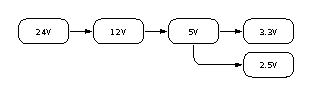
\includegraphics[width=.75\linewidth]{graphics/rail_hierarchy}
	\caption[Overview of the voltage rail hierarchy in the controller board design.]{Overview of the voltage rail hierarchy in the controller board design. The 24V rail is external and is used to genereate the 12V rail which generates the 5V rail which, finally, generates the 3.3V rail and 2.5V reference.}
	\label{fig:figure1}
\end{figure}

\begin{table}[h]
	\centering
	\begin{tabular}{r | r | r | r | r | r}
		Rail [V] & 24 & 12 & 5 & 3.3 & 2.5\\
		Accuracy [V] & $\pm$1 & $\pm$1 & $\pm$0.5 & $\pm$0.25 & $\pm$0.03\\
		Current [A] & 85 & - & 2.5 & 1 & -
	\end{tabular}
	\caption{Voltage rails to be created on the controller board and their specification.}
	\label{tab:powerrails}
\end{table}

\subsubsection{Motor Current Sensing}
In order to implement current mode control it is necessary to accurately measure the current being drawn by the motor at any given time.
Current measurements are generally done by either hall effect based sensors or shunt resistors. 
Hall effect based sensors are usually better for high current applications where adding a resistor in series with the load is infeasible. 
Additionally, their interference with the circuit they are measuring is negligible.
Hall effect sensors however, do come at a significant cost compared to the alternative described below.
A shunt resistor used for current measurements is simply a resistor with a very low resistance, typically $<$ 100m$\Omega$, and a high power rating ranging from a few watts into 10's of watts depending on the application.
By adding such a resistor in series with the load, the voltage across the resistor can be measured and from that the current through the load determined.
For this project a shunt resistor will be used since it is regarded as the simpler, cheaper option.

\subsubsection{Safety} % (fold)
\label{subsub:safety}
It is expected that, eventually, an error may occur that causes the cart to move uncontrollably.
A safety system should be constructed in such a way that it will prevent the cart from crashing violently or the electronics to self-destruct.
It should be isolated from the remaining system and no programming should be involved in determining whether a safety condition is met.
\\~\\
A safety condition is defined as a situation that, when not met, indicates that a critical or dangerous situation has occured with the system.
When a condition is met, that situation has not occured.
\\~\\
The safety system for this platform should be designed in such a way that, when activated, it will cut power to the motors.
In order to more easily identify the cause of the fault, the remaining electronics should remain operational to maintain the current program status.
Clearly, the system should function only if all safety conditions are met.
This will be ensured by creating an aggregation circuit which compares all of the safety conditions, creating one signal which will be capable of closing the main relay if necessary.
\\~\\
The system should be designed to have endstops.
These are in place to quickly cut power to the system if the cart reaches the end of the rail.
Creating these endstops can be done in different ways.
Three potential implementations are presented here:
\paragraph{Mechanical Switch:} % (fold)
\label{par:mechanical_switch}
The simplest form of switch is the mechanical switch.
The switch should be mounted in such a way that the cart would move into the switch, therefore activating it.
This approach is not without issues.
Mounting of the switch should be done in such a way that it is not in the direct path of the cart.
If the cart is traveling at full speed it is unlikely that the cart would stop before crashing into the switching mechanism.
A switch mounted in this fashion would need to be rather robust.
Some other mounting solutions could be thought of that do not suffer from this problem, especially if a flexible microswitch is used.
These would require significant extra design to properly mount the switch.
Mechanical switches can be fragile and may not be sufficiently durable, considering the usecase.
All mechanical switches have one drawback in common: they are mechanical and will be subject to wear over time, eventually requiring maintainance or replacement.

% paragraph mechanical_switch (end)
\paragraph{Hall Effect Sensor:} % (fold)
\label{par:hall_effect_sensor}
This type of sensor measures magnetic fields and produces a voltage proportional to the strength of the field.
By placing a small neodymium magnet on the cart and mounting a hall effect sensor on the rail in such a way that they coincide would allow for detecting when the cart is above the sensor.
If the sensor is combined with a schmitt-trigger circuit the output could be a binary result, either the endstop is reached or it is not.
Using this method requires that a magnet is placed on the cart itself and that a sensor is mounted to the rail.
It should be noted that accelerating rather strong magnetic fields back and forth on the platform may not be the least electrically noisy solution one could think of.
% paragraph hall_effect_sensor (end)
\paragraph{Infrared Transceiver:} % (fold)
\label{par:infrared_transceiver}
Infrared transceivers come in different configurations but generally the device is comprised of an LED and a photo transistor.
The LED is optimised for emitting infrared light, or radiation (IR).
In the configuration under consideration in this project the LED emits IR towards the photo transistor, opening it.
When an object passes between the LED and the transistor the transistor is closed.
This change can be detected using a simple schmitt-trigger circuit. 
With this sensor type it is important to realise that the LED will not be the only emitter of IR in the vicinity.
Any type of lamp will emit IR, especially glowbulbs but also sunlight contain a significant amount of IR.
When using this sensor the circuit should be designed in such a way that only the effect of the IR from the LED on the photo transistor will affect the circuit.
% paragraph infrared_transceiver (end)
\\~\\
While all of the above have their drawbacks, it was decided to use the infrared transceiver.
This sensor allows the greatest reliability while being reasonably simple to mount on the platform in that it requires no modification to the cart or rail.
\\~\\
In addition to the endstops, also an emergency button, preferably red, should be able to cut power to the motors.

\subsubsection{Schematic Revision} % (fold)
\label{ssub:schematic_revision}

% subsection schematic_revision (end)
From experience of the authors, a PCB layout is never error free in the first revision. 
This has been true even though a tremendous amount of work went into designing the PCB.
Therefore a strategy was devised to increase the likelihood of producing an error free PCB.
The strategy consist of five steps that needs to be completed after finishing the design of the board:

\begin{itemize}
	\item Documentation
	\item General inspection
	\item Datasheet and report comparison
	\item Footprint inspection 
	\item Peer-review
\end{itemize}

The content of each step will be elaborated here. 

\paragraph{Documentation:}
Each circuit should be documented to ensure that the design is done correctly.
Documenting a circuit requires studying the components datasheets and ensuring that they each meets the requirement.
Furthermore it requires a thorough inspection of the expected functionality of the circuit.
This step leads to correcting errors where a component is used incorrectly in respect to the desired functionality of the circuit.

\paragraph{General Inspection:}
General inspection of the schematic includes finding typographical errors on signals, components, resistor values, etc.
Furthermore each signal should be inspected to ensure that it is connected correctly and it should also be decided if it should be connected to an external header for measurement purposes.

\paragraph{Datasheet and Report Comparison:}
Each circuit in the schematic should be compared to its datasheets recommendation and the documentation written in the report. 
This step essentially ensures that each circuit has been verified more than one time. 
One could think that this step is irrelevant, but the authors believe it is important due to the complexity of the schematic.
After completion of this step, all circuits have been checked at least two times and the schematic should be correct. 

\paragraph{Footprint Inspection:}
Provided that the schematic is correct, the only possibly source of errors is the components footprints. 
Inspecting the footprint consist of verifying the correct pin assignment and the correct land patterns.
Both are done by inspecting the datasheet of each component. 
After completion of this step, both the schematic and footprints should be correct and the board is expected to be free from errors.

\paragraph{Peer-review:}
In this part of the process the board design, schematic and footprints should be correct and everything has been verified by the authors multiple times.
It is generally a problem that when working with a design for a long period of time, some errors are very hard to find for the designers themselves. 
Therefore the design should be reviewed by a person that has not taken part of the design of the board.
The review should be done by pointing out the main features of the board and discussing the found components, schematic and the board layout.

% section schematic_revision (end)

\subsubsection{PCB Layout} % (fold)
Some considerations are important when designing high power or switching circuitry, both of which are categories which the controller board fit into.
When part of the board is exposed to large currents, maintaining signal integrity on the remainder of the board becomes important.
This is done in large part by controlling grounds in the PCB.
An unbroken ground plane should be present in the design to ensure a low-impedance current path in the PCB \cite{pcblayoutds}.
In addition to unbroken ground planes, they should also be seperated based on their role in the circuit.
Often two, three or even more ground planes exist in circuits.
A common distribution is an analog ground, digital ground and power ground.
Analog signals are often sensitive to noise and should be shielded from the switching noise of the digital circuitry.
Similarly, high currents in a ground plane is likely to cause voltage drops across it.
This may cause issues in the digital circuitry.

Having several ground planes can cause issues with currents circulating in them.
In order to avoid this it is crucial that the ground planes are connected in one place only.
\\~\\
Since at least part of the PCB is likely to carry significant currents it is necessary to appropriately size the width of traces and the thickness of the copper.

\subsubsection{Component Selection and Placement} % (fold)
\label{ssub:component_case_selection_and_placement}
There are limits to the production capabilities of the equipment, both of the manufacturer producing the PCB and the equipment available to the authors at SDU.
For this reason some restrictions are set on the casing of components and their placement on a PCB.
Generally, throughhole components should be avoided where possible since these obstruct not only the layer they are placed on but also every other layer throughout the PCB and so surface mount technology (SMT) components are preferred.
SMT components come in many sizes and some are simply too small to realistically route and solder with the available equipment.
Generally, SOT-23, SOIC and 0805 packages and similar sizes are preferred where possible.
With the equipment available at SDU only components on one side of the PCB can be placed and soldered with the pick-and-place machine and oven.
Due to this, components should only be placed on the top layer when possible.
Larger components, such as big capacitors, can easily be hand-soldered and can therefore be placed on the bottom side of the PCB.
\\~\\
A number of signals should be routed to headers to allow for easier debugging and monitoring of the circuits.
For simplicity these headers should all be of the same type. 
The JST ZH-series connectors should be used as they are commonly used at SDU, they are SMT and sufficiently small. 


\subsubsection{Testing and Prototyping} % (fold)
Some of the developed circuits will consist of many components and complex ICs.
With such complex circuits, errors in a schematics can easily appear.
Therefore the functionality of the most important parts of the circuit should be tested on prototype PCBs before ordering an expensive PCB.

\subsubsection{Board Layout and Considerations} % (fold)
\label{ssub:board_layout_and_considerations}
A number of options are available when considering the general layout of the controller circuitry.
Different circuits can be segregated into individual boards, simplifying the layout and production of each board but imposing requirements on board-to-board connections between different circuits.
One possible configuration under consideration is the segregation of the digital circuit and the power circuits.
This would allow a different number of layers and different copper thickness on the two PCBs.
Extra layers are beneficial when routing the multitude of signals in a digital circuit but also add extra cost to the production of the circuit.
Similarly, extra copper is likely to be necessary on the power circuit but also adds cost.
Exploring various manufacturing options revealed that segregating the boards into one board with added copper and one board with added layers added significant cost to the order.
For this reason it was decided to produce just a single PCB with extra copper and four layers, housing all of the electronics related to the controller.

\clearpage
\subsubsection{Requirement Specification}

\paragraph{Functional:}
\begin{enumerate}[resume]
	\item Speed and direction of the motor should be adjustable through PWM from the MicroZed.
	\label{enum:motor_speed_direction}
	\begin{itemize}
		\item H-bridge of MOSFETs capable of switching motor current direction.
		\item H-bridge driver translating logic signals to gate signals.
		\item High side drive capabilities.
	\end{itemize}

	\item Motor current measurement through ADC input on the MicroZed.
	\label{enum:motor_current}
	\begin{itemize}
		\item Shunt resistor to measure the motor current.
	\end{itemize}

	\item Voltage rails for the various components in the circuit.
	\label{enum:voltage_rails}	
	\begin{itemize}
		\item 2.5V $\pm$0.03V.
		\item 3.3V $\pm$0.25V, 1A.
		\item 5V $\pm$0.5V, 2.5A.
		\item 12V $\pm$1V, The amperage of this rail should be as high as economically and practically viable.
		\item 24V $\pm$1V, 85A.
	\end{itemize}

	\item Voltage transients on voltage rails should be minimized.
	\label{enum:voltage_transients}	
	\begin{itemize}
		\item Bulk capacitors on 24V rail to supply current to motor.
		\item Properly sized input and output capacitance of DC/DC power supplies.
		\item Appropriate copper volume for ground and power wires.
	\end{itemize}

	\item The MicroZed should be correctly interfaced.
	\label{enum:microzed_interface}
	\begin{itemize}
		\item All signals to the MicroZed should be routed on the PCB to appropriate I/O ports.
		\item Start-up and shut-down power sequence and voltage levels should be correct.
	\end{itemize}
	\item A Heatsink should be connected to the MOSFETs to avoid overheating of the H-bridge.
	\label{enum:cool_mosfets}
	\item Hardware for wireless communication using RF should be implemented.
	\label{enum:hardware_for_wireless_implemented}
\end{enumerate}


\paragraph{Design:}
\begin{enumerate}[resume]
	\item Important parts of circuitry should be tested on prototype PCB.
	\label{enum:important_prototype}
	\item The PCB layout should be reviewed according to the developed strategy.
	\label{enum:pcb_strategy}
	\begin{itemize}
		\item Documentation.
		\item General inspection.
		\item Datasheet and report comparison.
		\item Footprint inspection.
		\item Peer-review.
	\end{itemize}
	\item The PCB layout should be designed with debugging in mind.
	\label{enum:pcb_debugging}
	\begin{itemize}
		\item Test points should exist for all voltage rails and relevant signals.
		\item All test points should be wired to JST ZH-series connectors.
	\end{itemize}
	\item The PCB layout should be designed to accomodate appropriate power levels.
	\label{enum:pcb_layout}
	\begin{itemize}
		\item Determine required trace width.
		\item Ground planes should be segregated for power and digital circuitry.
	\end{itemize}
	\item PCB soldering should be possible at SDUs facilities.
	\label{enum:pcb_soldering}
	\begin{itemize}
		\item Component casings should be SOT-23, SOIC or 0805 where possible.
		\item Avoid through-hole components.
	\end{itemize}
\end{enumerate}

\thomas{Needs mentioning: stall current, emergency signal from microzed, relays}
\paragraph{Safety:}
\begin{enumerate}[resume]
	\item Any triggered emergency condition should halt the cart.
	\label{enum:any_trigger_em}
		\begin{itemize}
			\item Emergency conditions should be implemented.
			\begin{itemize}
				\item[$\circ$] Emergency button for human interaction.
				\item[$\circ$] Endstops for detecting cart run-away.
				\item[$\circ$] Emergency signal from the MicroZed.
			\end{itemize}
			\item Relay should switch power to motor.
			\item Relay should be active only when emergency conditions are inactive.
			\item Power to remaining electronics and MicroZed should not be affected by an emergency condition.
		\end{itemize}
\end{enumerate}
